\section{Task 2 - And another screen}

\begin{frame}[containsverbatim]{Task 2 - And another screen}
    \begin{block}{Hint!}
        You can add properties to a widget and it's constructor

        \begin{minted}[fontsize=\footnotesize]{dart}
final String title;
const SecondScreen({super.key, required this.title});
        \end{minted}

        and access them in the State with, for example, \mint{dart}|widget.title|
    \end{block}
\end{frame}

\begin{frame}{Task 2 - And another screen}
    \begin{itemize}
        \item Create a second screen with the same layout as the first one, but that takes in the title as an argument
        \item Make the button on the first open the second
    \end{itemize}
\end{frame}

\begin{frame}{Task 2 - And another screen}
    \begin{columns}
        \begin{column}{0.5\textwidth}
            \begin{figure}[h]
                {
                    \setlength{\fboxsep}{0pt}%
                    \setlength{\fboxrule}{0.5pt}%
                    \fbox{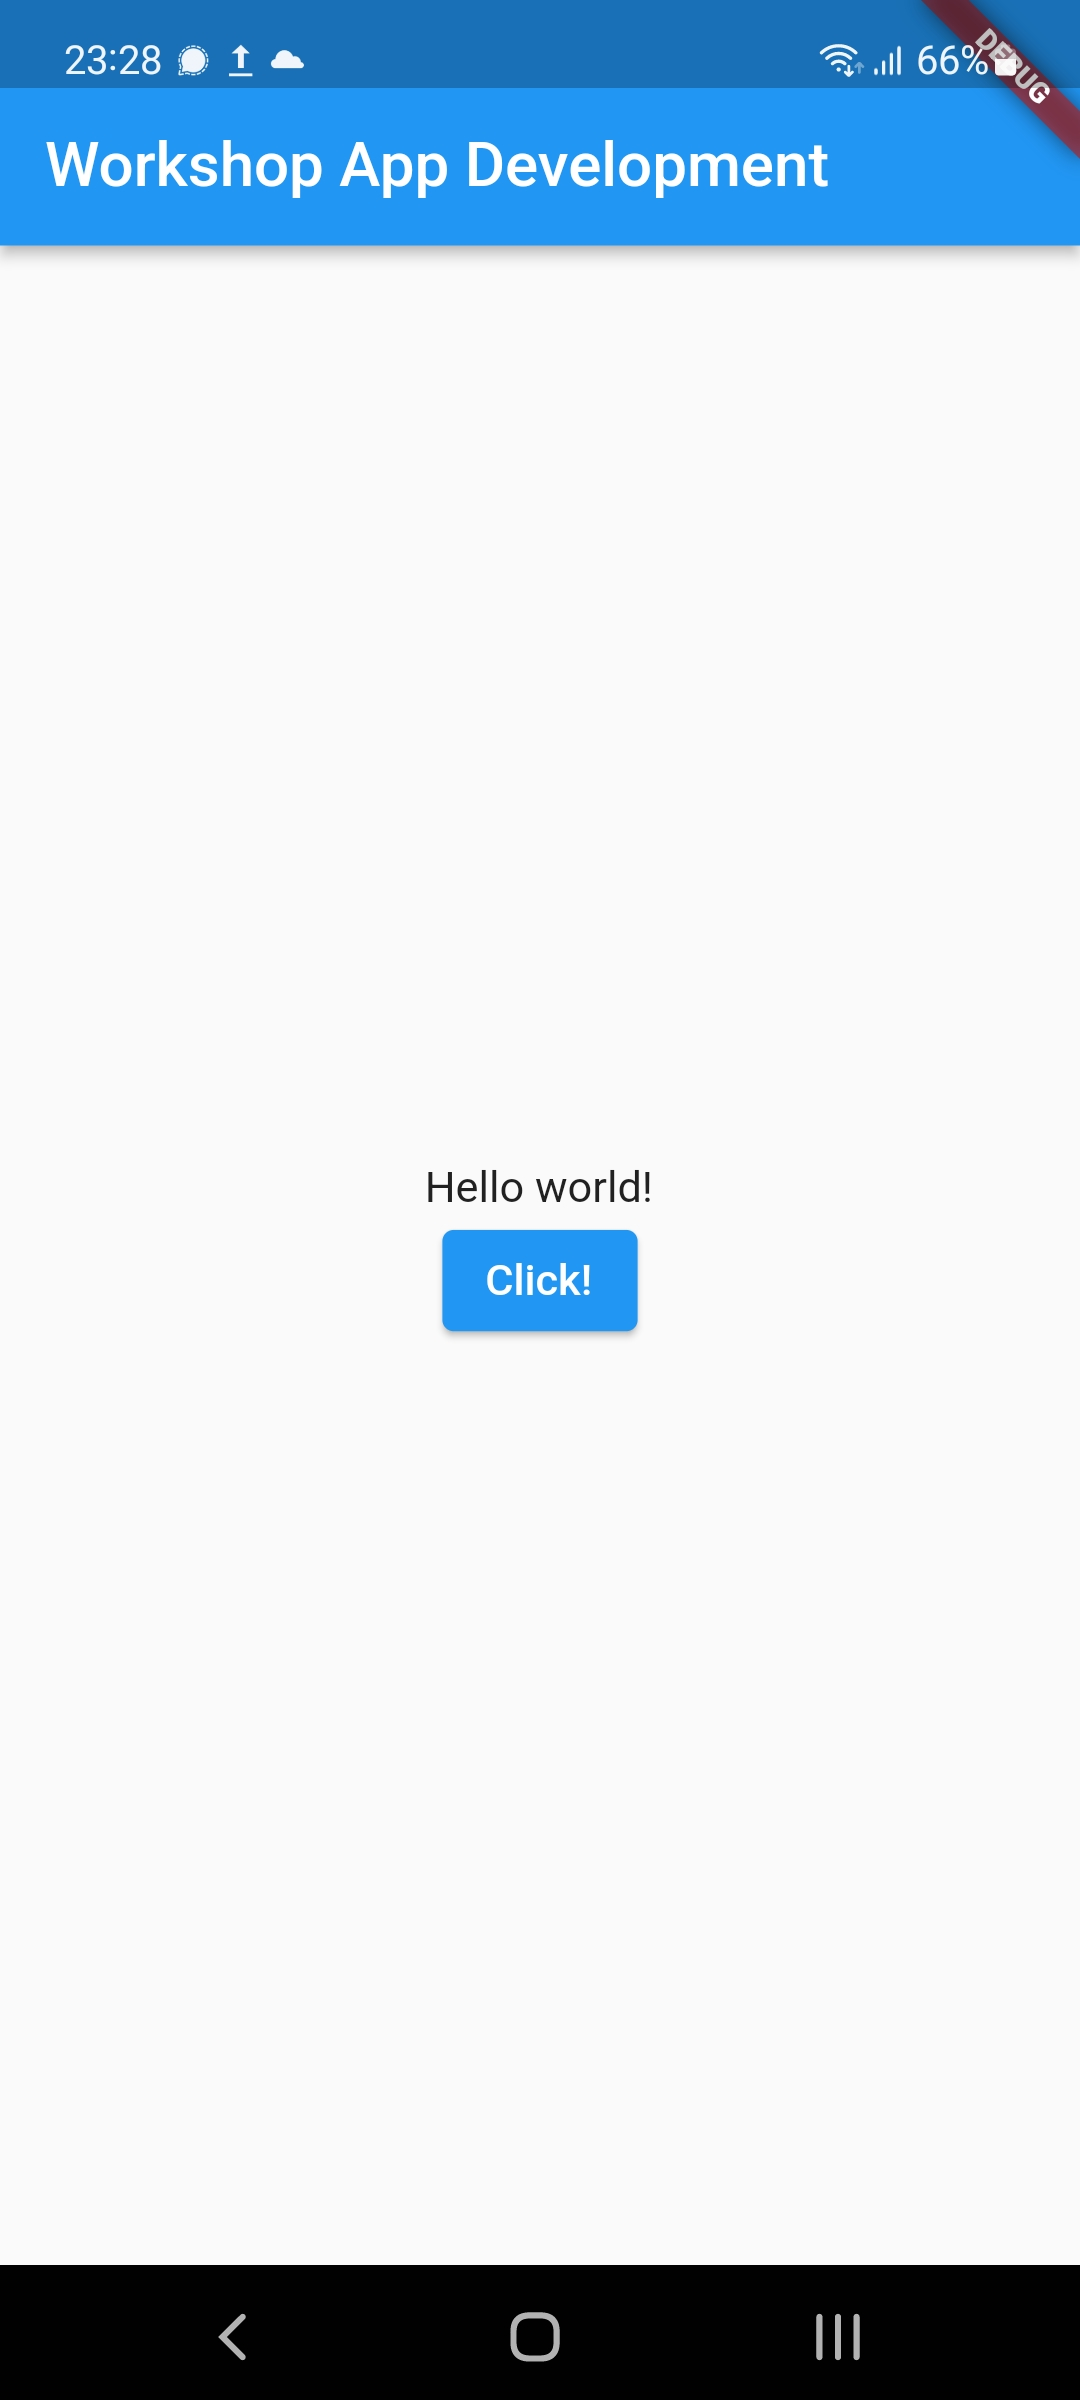
\includegraphics[width=0.5\textwidth]{images/task2-screen1.jpg}}
                }
            \end{figure}
        \end{column}
        \begin{column}{0.5\textwidth}
            \begin{figure}[h]
                {
                    \setlength{\fboxsep}{0pt}%
                    \setlength{\fboxrule}{0.5pt}%
                    \fbox{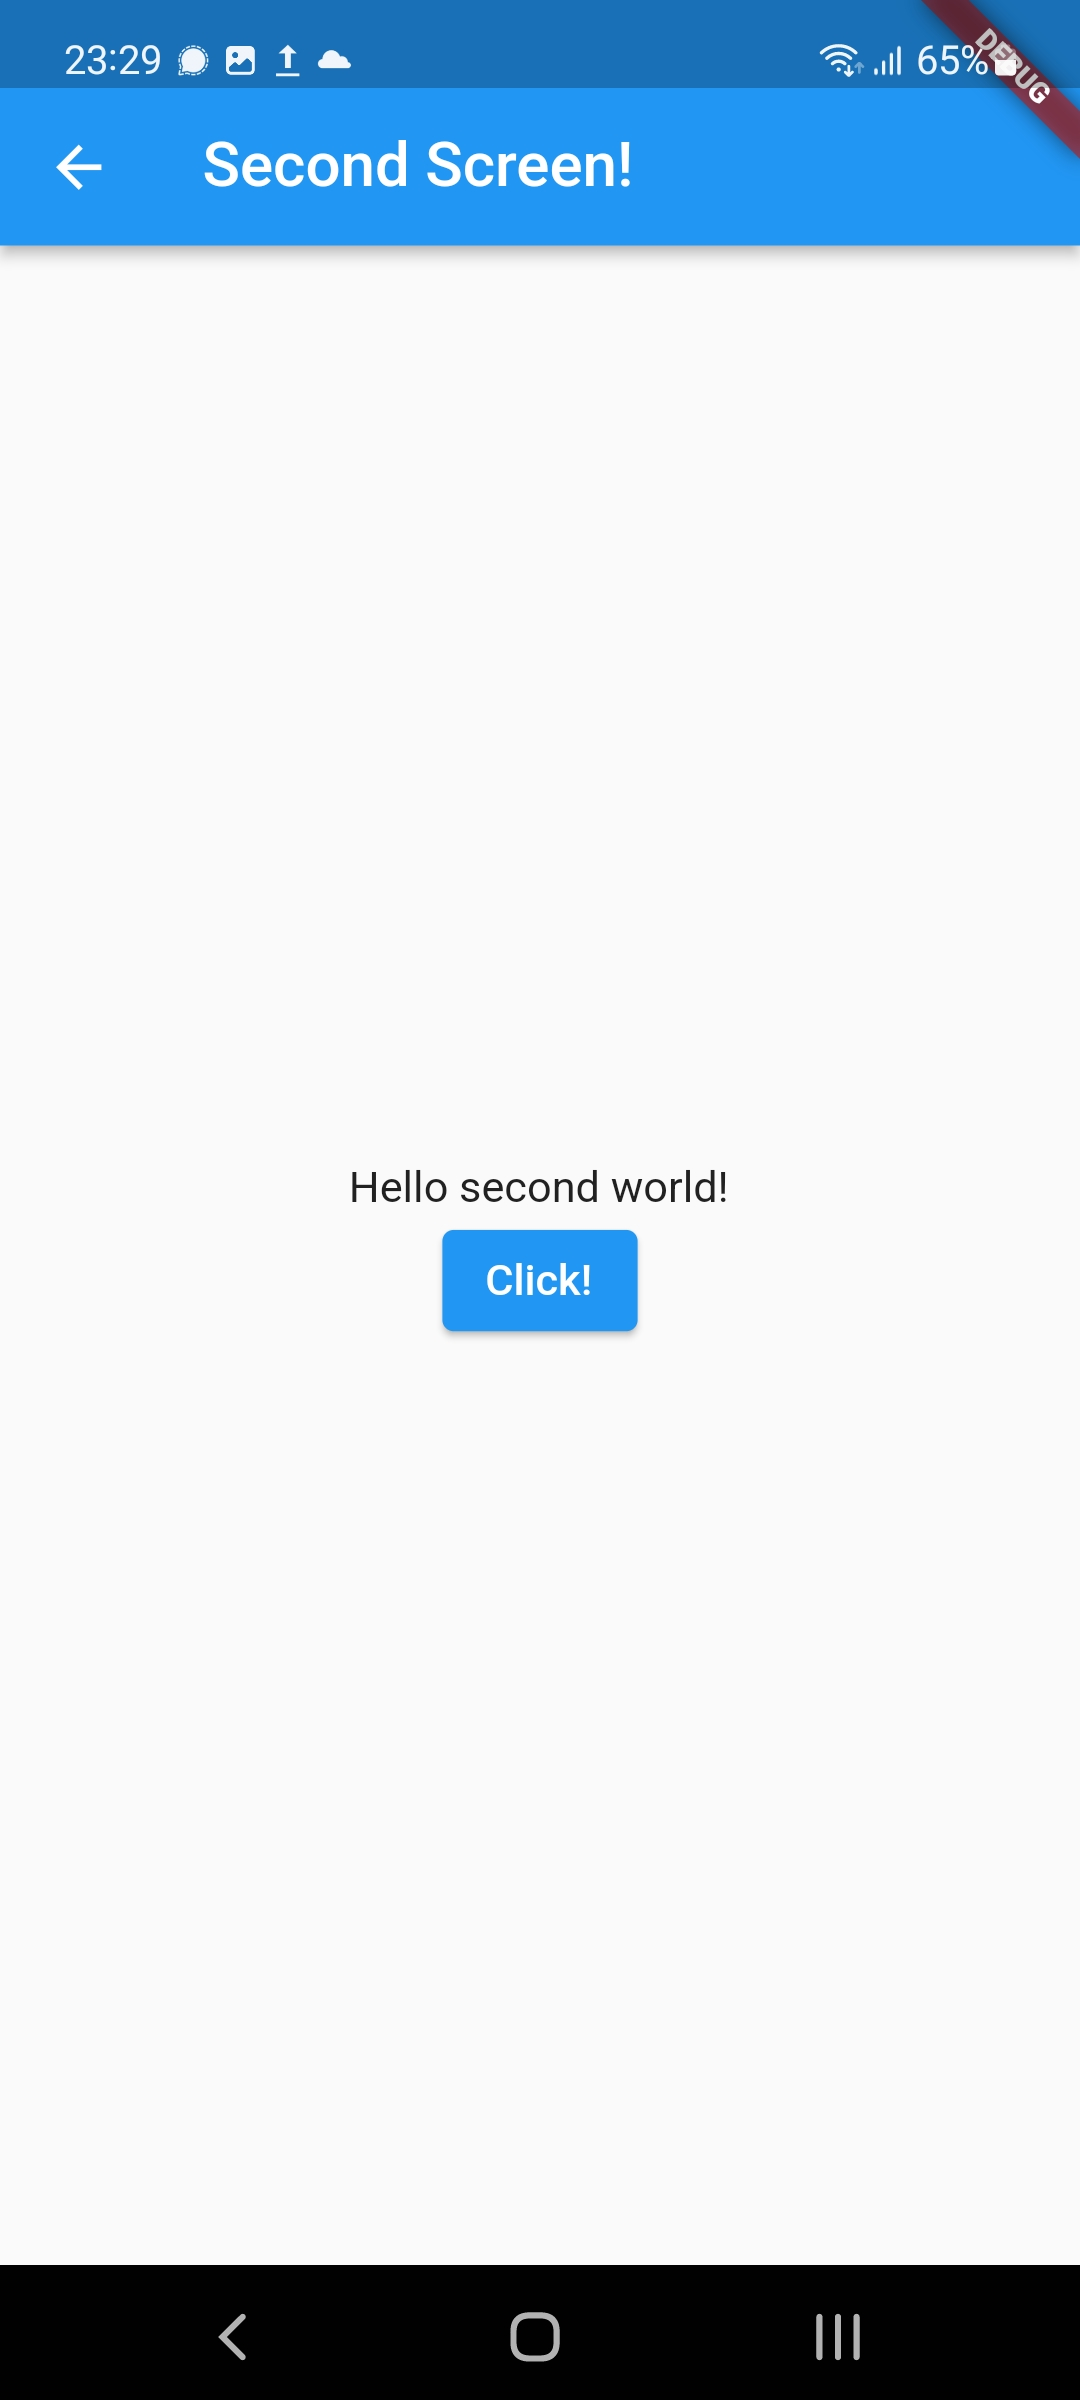
\includegraphics[width=0.5\textwidth]{images/task2-screen2.jpg}}
                }
            \end{figure}
        \end{column}
    \end{columns}
\end{frame}